\documentclass[conference]{IEEEtran}
\usepackage{amsmath}
\usepackage[utf8]{inputenc}
\usepackage{geometry}
\usepackage{xcolor}
\usepackage{tikz}
\usepackage{graphicx}

\geometry{margin=1in}  % Adjust page margins as needed

\begin{document}
\title{Project Proposal: Affordable Car Theft Detection and Alert System}
\author{\IEEEauthorblockN{Logan Paranto}}
\date{}
\maketitle

\begin{abstract}
This paper presents a project proposal for the development of an affordable car theft detection and alert system. The proposed system aims to enhance vehicle security by utilizing the STM32 microcontroller and the u-blox NEO-7M GPS module. This paper discusses the rationale behind the choice of components and outlines the potential impact of the project on enhancing vehicle security and convenience.
\end{abstract}

\section{Introduction}
This senior project aims to create a budget-friendly and efficient car theft detection and alert system for vehicles without advanced security. To do this, I've chosen the STM32 microcontroller and u-blox NEO-7M GPS module, and I'll use STM32CubeIDE for programming. These choices ensure top performance, affordability, and easy integration, providing a strong solution against car theft.

\section{Microcontroller Selection}
The STM32 microcontroller compared with two other options: the Arduino Uno and the PIC32 series, emerged as the best choice for our project.

Compared to the Arduino Uno, the STM32 offers more processing power and versatility due to its ARM Cortex-M architecture. It also provides a wide range of peripherals and has strong community support, making it adaptable to our project's needs.

In contrast to the PIC32 series, the STM32 is more power-efficient and easier to integrate. Its low power consumption aligns with our battery-powered design, and STM32CubeIDE simplifies software development and system integration, reducing complexity and development time.

In summary, the STM32 microcontroller's combination of performance, power efficiency, and community support makes it the ideal choice for our car theft detection and alert system, ensuring a reliable and cost-effective solution.

\begin{figure}
  \centering
  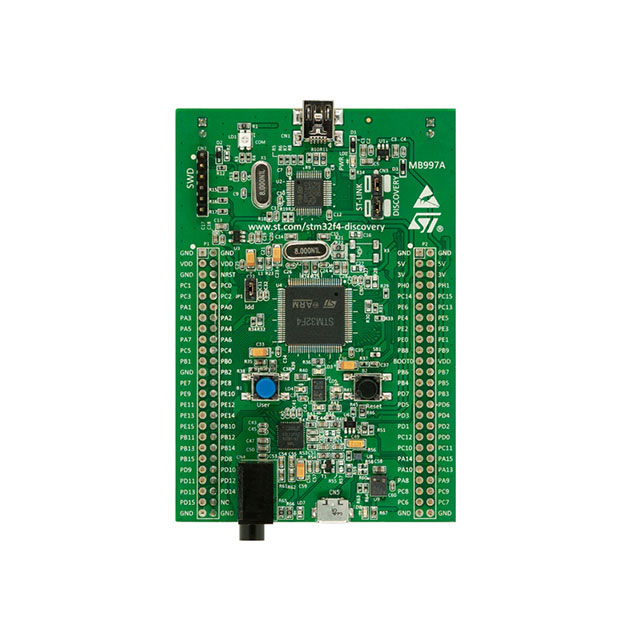
\includegraphics[width=0.7\columnwidth]{STM32.jpg}
  \caption{STM32 Microcontroller}
\end{figure}


\section{GPS Module Choice}
The u-blox NEO-7M GPS module was picked because it's known for being accurate and efficient. It can quickly pinpoint locations, making it great for real-time vehicle tracking. It's also power-efficient, which suits the battery-powered design. Plus, it works smoothly with STM32 microcontrollers, ensuring easy communication between them.

\begin{figure}
  \centering
  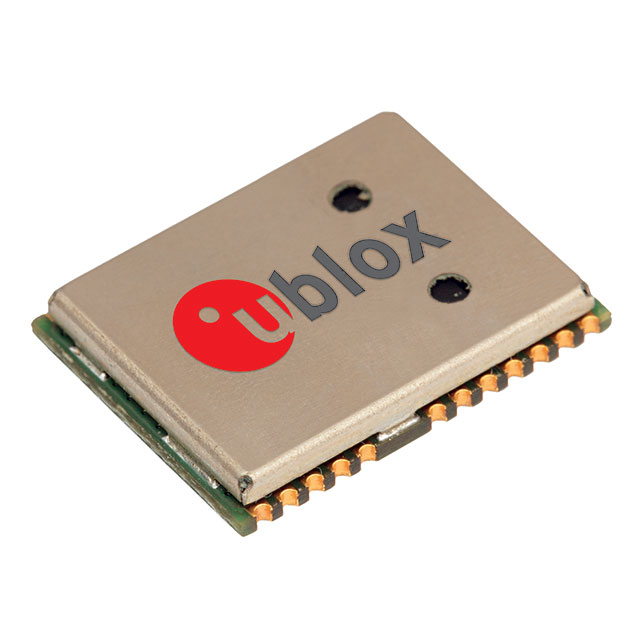
\includegraphics[width=0.7\columnwidth]{u-blox.jpg}
  \caption{u-blox NEO-7M GPS module }
\end{figure}

\section{Different Car Sensors Used Today}
Modern cars use various sensors for safety and functionality. These include ultrasonic sensors
for parking, motion detectors for alarms, accelerometers for stability, and pressure sensors for
tire safety. Microcontrollers like Arduino Mega, STM32, ATmega, MSP430, PIC, and others are
commonly used to process data from these sensors, depending on the specific application. Each
sensor serves a unique purpose, and the choice of microcontroller depends on sensor specifications and integration needs.

\section{Past Project References}
Previous projects have effectively utilized the STM32 microcontroller and u-blox GPS modules in
various applications. In weather stations, the STM32 helped collect data like temperature and
humidity, while the u-blox GPS module added location-specific weather information, enhancing
real-time weather forecasting.
In asset tracking systems, the STM32 was instrumental in monitoring valuable assets' location
and status. The u-blox GPS module provided real-time location updates and alerted in case of
unauthorized movements. These projects highlight the adaptability and reliability of our chosen
components in different applications, strengthening their suitability for the car theft detection
and alert system.

\section{Future Project Expansion}
In the future, this project can become even more appealing. Imagine having a smartphone app
that lets you effortlessly protect your car. With this app, you can monitor your car's security, get
quick alerts, and easily track its location in real-time. This upgrade not only boosts security but
also gives you more control and peace of mind. It's a valuable addition that makes this project
even more enticing for anyone who wants both security and convenience in one package.

\section{Conclusion}
In conclusion, the proposed project seeks to develop an affordable and effective car theft
detection and alert system using the STM32 microcontroller and u-blox NEO-7M GPS module.
These choices were made for their reliability, cost-effectiveness, and compatibility. The project
has the potential to enhance vehicle security and can be expanded into a mobile application,
providing car owners with comprehensive control and peace of mind.

\section{References}
\begin{thebibliography}{1}
    \bibitem{STMicroelectronics}
    STMicroelectronics. (n.d.). STM32 Microcontroller Portfolio.
    \texttt{https://www.st.com/en/microcontrollers-microprocessors/stm32-32-bit-arm-cortex-mcus.html}
    
    \bibitem{u-blox}
    u-blox. (n.d.). NEO-7M Product Page.
    \texttt{https://www.u-blox.com/en/product/neo-7-series}
    
    \bibitem{Community Forum}
    Community Forum - STMicroelectronics. (n.d.).
    \texttt{https://community.st.com/s/}
\end{thebibliography}

\end{document}
